%& C:\Users\lizil\AppData\Roaming\TikzEdt\TikzEdt\023~1.0\TEMP_H~1
\begin{document}
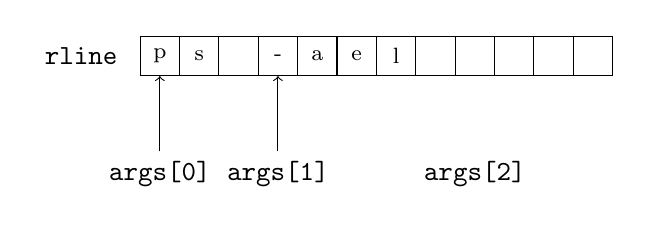
\begin{tikzpicture}
\tikzstyle{box} = [minimum width=0.5cm, minimum height=0.5cm, draw, font=\footnotesize];

\foreach \x/\y in {1/p,2/s,3/,4/-,5/a,6/e,7/l,8/,9/,10/,11/,12/}
	\node[box] (n-\x) at (\x*0.5,0) {\y};

\node at (-0.5,0) {\texttt{rline}};
\node (t-0) at (0.5,-1.5) {\verb"args[0]"};
\draw[->] (t-0) edge (n-1);
\node (t-1) at (2,-1.5) {\verb"args[1]"};
\draw[->] (t-1) edge (n-4);
\node at (4.5,-1.5) {\verb"args[2]"};

\usetikzlibrary{calc}
\pgftransformreset
\node[inner sep=0pt,outer sep=0pt,minimum size=0pt,line width=0pt,text width=0pt,text height=0pt] at (current bounding box) {};
%add border to avoid cropping by pdflibnet
\foreach \border in {0.1}
  \useasboundingbox (current bounding box.south west)+(-\border,-\border) rectangle (current bounding box.north east)+(\border,\border);
\newwrite\metadatafile
\immediate\openout\metadatafile=\jobname_BB.txt
\path
  let
    \p1=(current bounding box.south west),
    \p2=(current bounding box.north east)
  in
  node[inner sep=0pt,outer sep=0pt,minimum size=0pt,line width=0pt,text width=0pt,text height=0pt,draw=white] at (current bounding box) {
\immediate\write\metadatafile{\p1,\p2}
};
\immediate\closeout\metadatafile
\end{tikzpicture}

\end{document}

